\titre{Langage régulier :} Reconnu par un automate (déterministe ou non) ou donné par une expression régulière. Tous les langages ne sont pas réguliers!!! \\

\titre{Exemples :}
\begin{enumerate}
	\item Sur l'alphabet $\Sigma = \{ a \}$, $L = \{ a^{n^2},n\in\N \}$
	\item Sur l'alphabet $\Sigma = \{ a,b\}$, $L =$ ensemble des mots ayant autant de $a$ que de $b$\\
	\titre{Preuve :} \\
	Supposons qu'il existe un automate $A$ déterministe qui reconnait $L$. Soit $n$ le nombre d'états de $A$. Cet automate accepte $a^{n+1}b^{n+1}$. En lisant les $n + 1 a$, il y a forcément un moment où on repasse par un même état. Alors en cet état il y a deux sorties $a$, ce qui est impossible dans un automate déterministe. De plus, comme on ne sait pas le nombre de passage dans la boucle, il reconnaitrait forcément des mots contenant plus de $a$ que de $b$.\\
	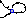
\includegraphics[width=100px]{Images/fig3.pdf}
	\item Sur l'alphabet $\Sigma = \{ a,b\}$, $L =\{a^nb^n, n\in \N\}$
\end{enumerate}
\newpage
\titre{Lemme de pompage :} Si un langage est régulier alors il existe un nombre $n$ avec la propriété suivante : Si $w$ est un mot du langaga de taille supérieure à $n$, alors $w=u_1u_2u_3$ avec $u_1u_2^*u_3$ est dans $L$ et la taille de $u_1u_3$ est inférieure ou égale à $n$. \\

\titre{Rq :} On l'utilise en général pour montrer qu'un langage n'est pas régulier.\\

\titre{Théorème de Myhill-Nerode :} Un langage est régulier ssi il a un nombre fini de dérivées.\\

\titre{Idée de preuve :}
\begin{itemize}
	\item nombre fini de dérivée $\impl$ automate des dérivées
	\item d'un automate déterministe donné il suffit de changer l'état initial pour avoir celui de la dérivée.
\end{itemize}
